% !Mode::"TeX:UTF-8"
\documentclass[UTF8]{article}   %this [UTF8] is very important
\usepackage{ctex}               %中文支持
\usepackage{fancyhdr}           %页眉页脚
\usepackage{geometry}           %调整页边距
\geometry{a4paper,left=2cm,right=2cm}
\usepackage{underscore}         %支持下划线作为文本输入
\usepackage{graphicx}           %支持图片插入
\usepackage{float}
\usepackage{amssymb}            %支持数学符号
\usepackage{xlop}               %支持竖式除法的排版
\usepackage{booktabs}           %支持表格的线
\usepackage{caption}            %设置字体
\usepackage{listings}           %支持代码
\usepackage{varwidth}           %支持图片顶部对齐
\usepackage{amsmath}            %支持多行公式的数学环境
\usepackage{epstopdf}           %支持pdfLatex下用eps
\usepackage{multirow}           %支持合并单元格
\usepackage{longtable}          %支持长表格
\usepackage{appendix}
\usepackage{colortbl}           %支持彩色表格
\usepackage{color}

\chead{\thesection}
\cfoot{\thepage}
\author{朱德森}
\title{解题思路}
\begin{document}
\songti
\linespread{1.3}
\maketitle
%\tableofcontents
\newpage

\section{解题思路}
傅里叶派赛题可以看做矩阵中找圈4,6,8,10,12,14。本方案是以坐标的角度解题,则该圈需要满足一定的条件,即所有的顶点的横坐标和纵坐标必须且只能出现2次,满足该条件即可满足画圈方式不同。
另外,题目中规定木托盘上出现的人名不能重复,
即需要在画圈之后对结果中的横坐标纵坐标进行重复判断,排除所得到的的圈中的重复圈,
即得到结果。

\section{具体方案}
\subsection{CSV文件读取}
利用strtok函数对读取到的csv文件的某行根据逗号分隔,
并将数值存储入二维数组中暂存。
得到矩阵大小和矩阵之后,
分别将每一行,每一列中数值1的数量和位置索引
存入Edge结构体中备用。

\subsection{圈的寻找}
本方案中圈的寻找可以类比于贪吃蛇游戏,
初始化时需要设定2个点作为起始,一个称为Head,一个称为Tail。
为了防止循环时重复检测,令Head和Tail的横坐标相同,
并且设定Head和Tail所处的竖线为最左边的竖线。

设当前寻找的圈长为CircLen,则易得,当寻找到一个正确的圈时,
其所有的纵坐标的种类(即不同的纵坐标值)数量为CircLen/2。
整个过程可以简化为寻找新的纵坐标点的过程。

本方案的坐标点寻找过程如图{\ref{HeadMove}}所示,
其中坐标的移动是根据Edge结构体中存的索引进行。
\begin{figure}[H]
  \centering
  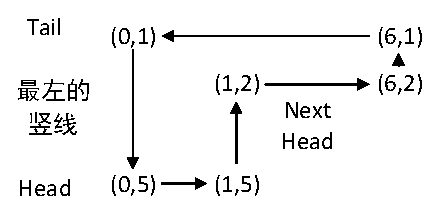
\includegraphics[width=0.4\textwidth]{./pic/HeadMove}
  \captionsetup{font={small}}
  \caption{坐标点搜寻过程示意图}
  \label{HeadMove}
\end{figure}

注意到Tail在寻找过程中是保持不变的,
因此可以提前算出Tail所在纵坐标的所有点的信息,
此处本方案计算某一列与Tail所在纵坐标的差值,
并保存在二叉树中,方便后续反复查询。
在寻找最后两个坐标点的时候,可以算出当前Head和Tail之间纵坐标的差值,
通过在二叉树中查询是否存在此差值,即可判断该圈是否可以收尾。


\begin{enumerate}
  \item 设定Head和Tail
  \item Head横向移动寻找不同的横坐标
  \item Head纵向移动寻找不同的纵坐标
  \item 若剩余需寻找的新纵坐标数为0,下一步,否则跳转至2
  \item Head和Tail横向移动寻找相同横坐标的点收尾
\end{enumerate}

其中需要对横坐标,纵坐标是否重复进行判断,
对此设置了堆栈进行辅助。

\subsection{名字重复判断}
在所搜寻的圈中,可能会出现图{\ref{RepeatName}}中所示的情况,
此时圈不同,但是其名字是重复的,两种应该算作一种情况。

\begin{figure}[H]
  \centering
  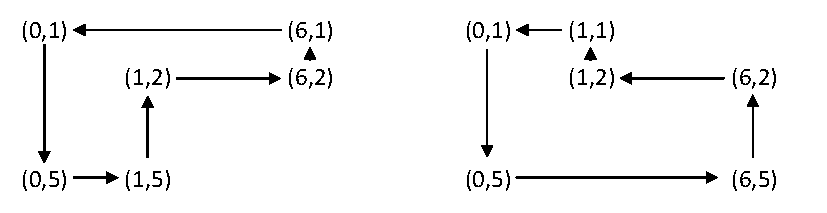
\includegraphics[width=0.9\textwidth]{./pic/RepeatName}
  \captionsetup{font={small}}
  \caption{圈不同但名字重复}
  \label{RepeatName}
\end{figure}

创建一个结果矩阵对历史结果进行存储,为二维矩阵。
计算所得到的圈的横坐标之和与纵坐标之和作为结果矩阵的索引。
当得到一个圈时,在二维矩阵中寻址,若该位置未存过结果,
则以链表方式存入。
若已经存入结果,则需要与历史结果比较,判断是否重复,
重复则忽略此圈,否则存入当前链表。

由于本方案中已经设定了初始的两个坐标构成了最左的竖线,
因此当竖线右移时候,结果矩阵中的前几列不会再出现,
因此可以提前释放前几列中存放的结果,以节省内存。





\end{document} 